\section{Aufgabenstellung}
In diesem Versuch sollen die Halbwertszeiten von $^{147}Sm$ (Samarium-147) und $^{40}K$ (Kalium-40) bestimmt werden. Da deren Halbwertszeiten sehr hoch sind, kann die zeitabhängige Änderung der Impulsrate nicht beobachtet werden. Stattdessen muss die Aktivität A und die Zahl der radioaktiven Atome N, welche eine messbare Strahlung absondern, bestimmt werden und mithilfe dieser Größen durch $T_{1/2}=ln(2)\frac{N}{A}$ die Halbwertszeit jeweils bestimmt werden.
\section{Theoretische Grundlagen}
\subsection{Zerfallsarten}
Es wird grundsätzlich zwischen drei Arten von radioaktiver Strahlung unterschieden.
\subsubsection{$\alpha$-Strahlung}
Bei dieser Strahlung zerfällt der Mutterkern $^{A}_{Z}X$ mit Massenzahl A (Anzahl an Protonen und Neutronen im Kern) und Kernladungszahl Z (Anzahl Protonen im Kern) unter Aussendung eines zweifach positiv geladenen Heliumkerns $^{4}_{2}He^{2+}$ zu dem zweifach negativ geladenen Tochterkern $^{A-4}_{Z-2}Y^{2-}$, wobei Energie frei wird, wie folgender Gleichung entnommen werden kann: \[^{A}_{Z}X\rightarrow ^{A-4}_{Z-2}Y^{2-}+^{4}_{2}He^{2+}+\Delta E\]
Die freiwerdende Energie hängt von den Reaktionskernen ab und ist diskret. Typischerweise hat die $\alpha$-Strahlung eine Energie im Bereich einiger MeV (Quelle: [wis]). Da die ausgesandten $^{4}_{2}He^{2+}$-Kerne elektrisch geladen und ziemlich schwer sind, ist die Reichweite dieser Strahlung sehr gering (in Luft wenige cm (Quelle: [wis])). Bereits ein Blatt Papier reicht aus, um $\alpha$-Strahlung abschirmen zu können.
\subsubsection{$\beta$-Strahlung}
Bei der $\beta$-Strahlung bleibt die Massenzahl konstant und die Ladungszahl ändert sich um eine Einheit. Es gibt drei Arten von Zerfällen, welche zur $\beta$-Strahlung gezählt werden:\\
\textbf{\uline{$\beta^{-}$-Zerfall}}
\[^{A}_{Z}X\rightarrow ^{A}_{Z+1}Y+e^{-}+\overline{\nu_{e}}.\] Ein Neutron wandelt sich also in ein Proton um (die Kernladungszahl Z wird um 1 erhöht) und emittiert dabei ein Elektron ($e^{-}$) und ein Anti-Neutrino ($\overline{\nu_{e}}$): \[n\rightarrow p+e^{-}+\overline{\nu_{e}}.\]
\textbf{\uline{$\beta^{+}$-Zerfall}}
\[^{A}_{Z}X\rightarrow ^{A}_{Z-1}Y+e^{+}+\nu_{e}.\]
Hierbei wandelt sich ein Proton unter Emission eines Positrons $e^{+}$ und eines Neutrinos $\nu_{e}$ in ein Neutron um: \[p\rightarrow n+e^{+}+\nu_{e}.\] Die Kernladungszahl verringert sich dabei um eine Einheit.\\
~\\
~\\
~\\
~\\
\textbf{\uline{Elektroneneinfang / Electron Capture}}\\
Bei dem Elektroneneinfang handelt es sich um einen Konkurrenzprozess zum $\beta^{+}$-Zerfall, da der jeweilige Mutterkern in denselben Tochterkern verwandelt wird wie bei diesem. Auch hier wird die Kernladungszahl also um eine Einheit verringert.
Es wird ein Bahnelektron (meist aus der K-Schale, alternativ aus anderen kernnahen Schalen) unter Emission eines Neutrinos vom Kern eingefangen. Dabei kommt es zur Umwandlung eines Protons in ein Neutron. \[p+e^{-}\rightarrow n+\nu_{e}\]
\[\Leftrightarrow ^{A}_{Z}X+e^{-}\rightarrow ^{A}_{Z-1}Y+\nu_{e}.\]
\textbf{\uline{Eigenschaften}}\\
$\beta$-Strahlung hat im Gegensatz zu $\alpha$-Strahlung keine fest vorgegebene Energie, sondern ein kontinuierliches Spektrum an möglichen Energien, da die beim Zerfall frei werdende Energie auf den Atomkern, das Elektron/Positron und das Antineutrino/Neutrino verteilt wird. Dabei gibt es eine Maximalenergie, welche vom zerfallenden Kern abhängt. Typischerweise liegt diese in der Größenordnung von keV bis einigen MeV. Zur Abschirmung von $\beta$-Strahlung muss mindestens ein dünnes Blech verwendet werden. Die Reichweite von $\beta$-Strahlung in Luft beträgt einige Meter (Quelle: [bstr]).
\subsubsection{$\gamma$-Strahlung}
Diese Art der radioaktiven Strahlung ändert weder die Massen-, noch die Ladungszahl eines Kerns. Sie beschreibt das Aussenden von elektromagnetischer Strahlung, wenn ein angeregter Kern in sein energetisches Grundniveau zurückfällt. Bei Zerfallsprozessen tritt die $\gamma$-Strahlung als Begleiterscheinung nach einem $\alpha$- bzw $\beta$-Zerfall auf. Da sie aus Photonen besteht, ist sie elektrisch neutral.
\subsection{Wechselwirkung geladener Teilchen mit Materie}
Der Nachweis geladener Teilchen wird durch elektromagnetische Wechselwirkungen ermöglicht. Die hauptsächlich dafür verantwortlichen Vorgänge sind Ionisation, Anregung und Bremsstrahlung. 
\subsubsection{Anregung und Ionisation}
Beim Durchgang von geladenen Teilchen durch Materie kommt es zu Stößen mit Atomen und Molekülen. Dabei werden diese auf ein höheres Niveau angeregt oder ionisiert (es werden Elektronen aus dem Atom bzw. Molekül herausgeschlagen). Maximal kann bei einem Stoß die Energie $E_{max}=2m_{e}c^{2}\beta^{2}\gamma^{2}=2m_{e}v^{2}\gamma^{2}$ (Quelle:[sta]) übertragen werden. Dabei ist $m_{e}$ die Elektronenmasse, $\beta=\frac{v}{c}$ die Geschwindigkeit des Teilchens relativ zur Vakuumlichtgeschwindigkeit und $\gamma=\frac{E}{m_{0}c^{2}}$ der sogenannte Lorentzfaktor. \\
Im Hinblick auf den resultierenden Energieverlust gibt es einen großen Unterschied zwischen $\alpha$- und $\beta$-Strahlung: Erstere erzeugt pro cm Luft etwa 30000 Ionenpaare, während letztere etwa 50 bis 1000 erzeugt (Quelle: [sta]).
\subsubsection{Bremsstrahlung}
Im Coulombfeld der Kerne verlieren geladene Teilchen Energie. Dadurch werden sie abgebremst und strahlen einen Teil ihrer Energie als Photonen ab. Für hohe Energien gilt dabei: \[-\frac{dE}{dx}=\frac{E}{x_{0}}\] Durch diese Gleichung wird die Energieänderung durch Bremsstrahlung nach der Schichtdicke x beschrieben. $x_{0}$ ist die Schichtdicke, nach der die Energie E auf den $1/e$-ten Anteil der Anfangsenergie abgefallen ist.
\subsection{Absorption und Reichweite radioaktiver Strahlung}
Die Reichweite radioaktiver Strahlung ist die Strecke, nach der ein Teilchen seine Energie vollständig verloren hat: \[R=\int_{E}^{0}-\frac{dE}{dE/dx}\]
Wie bereits erwähnt, ist die Reichweite von $\alpha$-Strahlung sehr gering und kann schon durch ein Blatt Papier oder wenige cm Luft abgeschirmt werden. Für die Abschirmung von $\beta$-Strahlung benötigt man dagegen eine dünne Bleischicht (ca. 1 mm). In Luft kommt diese Strahlung mehrere Meter weit.
\subsubsection{Selbstabsorption}
Wenn, wie in diesem Versuch, radioaktive Strahler untersucht werden sollen, muss beachtet werden, dass innerhalb der Probe emittierte Strahlung wieder von dieser absorbiert werden kann. \\
Dieser Effekt ist besonders bei $\alpha$-Strahlung von Bedeutung: Da diese nur eine sehr kurze Reichweite hat, wird nicht das komplette Volumen des Strahlers berücksichtigt, sondern nur die Oberfläche und die Reichweite, welche die maximale Schichtdicke beschreibt, da die von den darunter liegenden Schichten emittierte $\alpha$-Strahlung von den anderen Atomschichten absorbiert wird.\\
Bei $\beta$-Strahlung tritt dieser Effekt aufgrund der erheblich größeren Reichweite deutlich schwächer auf. Aus diesem Grund wird für den $\beta$-Strahler die Zählrate für unterschiedliche Massen der Probe bestimmt.
\subsection{Gasionisationsdetektoren}
Um $\alpha$- bzw. $\beta$-Strahlung nachzuweisen, verwenden wir in diesem Versuch einen Gasionisationsdetektor. In diesem wird durch zwei Elektroden ein elektrisches Feld erzeugt. Einfallende Teilchen oder Strahlung ionisieren die Atome bzw. Moleküle des darin befindlichen Gases (in diesem Versuch Methan ($CH_{4}$)). Die negativ geladenen Elektronen driften zur Anode, die positiv geladenen Ionen zur Kathode. An den Kontakten wird dadurch eine Ladung induziert, welche über einen Wechselkopplungskondensator und einen Vorverstärker in einen Spannungsimpuls umgewandelt wird. Da die induzierte Ladung proportional zur Zahl der ankommenden Elektronen bzw. Ionen ist, ist eine Proportionalität zwischen dem elektrischen Ausgangssignal und dem Energieverlust der einfallenden Teilchen gegeben. Aus diesem Grund spricht man von einem 'Proportionalzählrohr'. Der in diesem Versuch verwendete Detektor hat die Form eines Hohlzylinders, da so aufgrund seiner $1/r$-Abhängigkeit ein sehr starkes elektrisches Feld erzeugt werden kann, sodass das einfallende Teilchen möglichst seine gesamte Energie abgibt und diese dadurch genauer vermessen werden kann.\\
\clearpage
\subsection{Verwendete Proben}
\subsubsection{Natururanpräparat $^{238}U$}
Dieses Präparat wird verwendet, um die Zählrohrcharakteristik aufzunehmen. Uran bietet sich dabei an, da es $\alpha$- wie $\beta$-Strahlung emittiert und es zu sehr vielen Zerfällen kommt, weswegen nicht lange gemessen werden muss, um ein gutes Ergebnis zu erhalten. $^{238}U$ hat eine lange Zerfallsreihe, welche in $^{206}Pb$ (Blei) resultiert. 
\begin{figure}[h]
\begin{center}
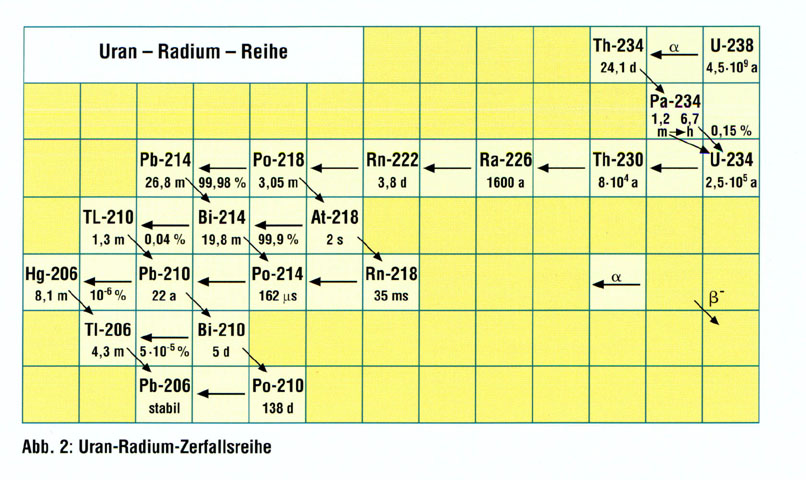
\includegraphics[scale=0.6]{Bilder/uran}
\caption{Zerfallsreihe $^{238}U$, Quelle: [uwa].}
\end{center}
\end{figure}
Wie der Zerfallsreihe entnommen werden kann, kommt es zu zahlreichen Zerfällen, bis ein stabiler Zustand erreicht wird, allerdings sind diese für den Versuch von keiner besonderen Bedeutung. \\
Die Halbwertszeit von $^{238}U$ beträgt $4,5\cdot10^{9}$ Jahre (s. Zerfallsreihe).
\subsubsection{Samariumpräparat $^{147}Sm$}
In dem Versuch verwenden wir Samariumdioxid $Sm_{2}O_{3}$, welches als Pulver mit 99\%-iger Reinheit vorliegt. $^{147}Sm$ ist ein $\alpha$-Strahler: Es zerfällt mit einer Übergangswahrscheinlichkeit von 100\% unter Emission von $\alpha$-Strahlung zu $^{143}Nd$, einem stabilen Isotop von Neodym. Das ausgestrahlte $\alpha$-Teilchen hat eine Energie von $2,233 MeV$ (Quelle: [sta]). Die Halbwertszeit von $^{147}Sm$ beträgt $1,06\cdot10^{11}$ Jahre (Quelle: [ver]). 
\subsubsection{Kaliumpräparat $^{40}K$}
In dem Versuch wird pulverförmiges Kaliumchlorid (KCl) verwendet. Es können zwei unterschiedliche Prozesse stattfinden: $\beta^{-}$-Zerfall bzw. Elektroneneinfang. Ersterer Prozess findet mit einer 89,28\%-iger Wahrscheinlichkeit statt und erzeugt Elektronen mit einer maximalen Energie von 1312 keV (Quelle: [sta]). \[^{40}_{19}K\rightarrow ^{40}_{20}Ca+e^{-}+\overline{\nu_{e}}\]Die Wahrscheinlichkeit für den Elektroneneinfang ist demnach 10,72\%. Mit einer Wahrscheinlichkeit von 10,67\% entsteht dabei Argon-40 im angeregten Zustand, wodurch es bei der Abregung in den Grundzustand zur Emission von (nicht detektierbarer) $\gamma$-Strahlung kommt. Mit einer Wahrscheinlichkeit von 0,05\% entsteht direkt Argon-40 im Grundzustand (für die Wahrscheinlichkeiten siehe [sta]).
\[^{40}_{19}K+e^{-}\rightarrow ^{40}_{18}Ar+\nu_{e}\]
 Es kommt also durch den Elektroneneinfang zu keiner nachweisbaren Strahlung. Dennoch muss diese bei der Bestimmung der Halbwertszeit von $^{40}K$ berücksichtigt werden (s. 'Mathematische Beschreibung'). Die Halbwertszeit von $^{40}K$ beträgt $1,28\cdot10^{9}$ Jahre (Quelle: [ver]).
 \subsection{Mathematische Beschreibung}
 \subsubsection{Halbwertszeit}
 Die Halbwertszeit beschreibt die Zeit, nach welcher die Zahl der anfänglich vorhandenen Nukliden durch Zerfall auf die Hälfte gesunken ist. Die Zahl der Nuklide in Abhängigkeit von der Zeit lässt sich beschreiben durch \[N(t)=N_{0}\cdot e^{-\lambda t}.\] Dabei ist $N_{0}$ die Zahl der anfänglich vorhandenen Kerne, t die Zeit und $\lambda$ die Zerfallskonstante, welche eine Wahrscheinlichkeit der Umwandlung pro Zeiteinheit angibt. Für die Halbwertszeit muss also gelten: \[N(T_{1/2})=0,5N_{0}\]
 \[\leftrightarrow N_{0}\cdot e^{-\lambda T_{1/2}}=0,5N_{0}\]
 \[\leftrightarrow -\lambda T_{1/2}=ln(0.5)=-ln(2)\]
 \[\leftrightarrow T_{1/2}=\frac{ln(2)}{\lambda}.\]
 \subsubsection{Aktivität}
 Die Aktivität beschreibt die Anzahl der Kernzerfälle pro Zeiteinheit. Für sie gilt: \[A(t)=-\frac{dN(t)}{dt}=\lambda N(t)\]
 Somit gilt: \[T_{1/2}=\frac{ln(2)}{\lambda}=\frac{ln(2)\cdot N}{A}.\]
  \subsubsection{Anwendung auf $^{40}K$}
   $^{40}K$ zerfällt unter Emission von $\beta$-Strahlung. Die Zählrate hat aufgrund der endlichen Reichweite der $\beta$-Strahlung eine Schranke und kann folgendermaßen modelliert werden: \[n(m)=a(1-e^{-bm}),\] wobei bei Ausschreiben von a und b diese zu \[n(m)=f_{B}\frac{\Omega}{4\pi}\frac{A}{m}\frac{F\rho}{\mu}\left(1-e^{\frac{-\mu\cdot m}{F\rho}}\right).\] Dabei gilt: $\mu$ ist der Abschwächungskoeffizient für $\beta$-Strahlung, $\Rho=2\pi$ ist der Raumwinkel, in welchem der Detektor funktioniert und $f_{B}=1,29$ (Quelle: [ver]) ist der Rückstreufaktor, mit der die Rückstreuung von Elektronen am Al-Schälchen berücksichtigt wird. \\
   Berücksichtigt man die Steigung der Tangente bei $m=0kg$, \[\frac{dn}{dm}=a\cdot b,\] so erhält man mithilfe des Rückstreufaktors und dem Faktor 2, welcher dadurch zustandekommt, dass nur $2\pi$ von insgesamt $4\pi$ des Raumwinkels abgedeckt werden, für die spezifische Aktivität: \[A_{s}=\frac{A}{m}=\frac{2ab}{f_{B}}.\] Die Teilchenzahl der $^{40}K$-Kerne wird berechnet durch \[N=\frac{h_{rel}m\cdot N_{A}}{m_{rel_{KCl}}}.\] Dabei ist $h_{rel}=1,18\cdot10^{-4}$ (Quelle: [ver]) der relative Massenanteil von $^{40}K$ in natürlichem Kalium und $m_{rel_{KCl}}=74,551\frac{g}{mol}$ (Quelle: [wal]) gilt. \\
   Für die Halbwertszeit gilt im Allgemeinen: \[T_{1/2}=\frac{ln(2)}{\lambda}.\] Nun muss hier, wie bereits erwähnt, berücksichtigt werden, dass es zum Elektroneneinfang kommen kann: Dieser Vorgang kann mit dem hier verwendeten Aufbau nicht detektiert werden. Aus diesem Grund gilt: \[\lambda=\lambda_{\beta}+\lambda_{EC}=\lambda_{beta}+\frac{10,72\%}{89,28\%}\lambda_{\beta}=1,12\lambda_{\beta}.\] 
   Für die Halbwertszeit gilt dann: \[T_{1/2}=\frac{ln(2)}{1,12}\frac{N}{A}=\frac{ln(2)}{1,12}\cdot\frac{h_{rel}f_{B}\cdot N_{A}}{2ab\cdot m_{rel_{KCl}}}=\frac{ln(2)\cdot h_{rel}N_{A}}{1,12\cdot m_{rel_{KCl}}A_{s}}.\]
 \subsubsection{Anwendung auf $^{147}Sm$}
 Wie bereits diskutiert, zerfällt $^{147}Sm$ unter Emission von $\alpha$-Strahlung. Diese hat eine begrenzte Reichweite $R_{Sm_{2}O_{3}}$. Die Zerfallsrate $n=\frac{N}{t}$ ist somit gegeben durch \[n=A_{V}\frac{F}{4}R_{Sm_{2}O_{3}},\] wobei $A_{V}=\frac{A}{V}$ die Aktivität pro Volumen Probe ohne Selbstabsorption darstellt. F gibt die Größe der Oberfläche an.\\
  Da $R_{Sm_{2}O_{3}}$ ebenso wie die Dichte des Stoffes $\rho$ unbekannt ist, kann deren Produkt ersetzt werden mithilfe der Beziehung von Bragg und Kleeman: 
  \[R\cdot\rho=C\sqrt{m_{A}}.\] C ist eine stoffunabhängige Proportionalitätskonstante, $m_{A}$ das effektive Atomgewicht. Um die Konstante C eliminieren zu können, muss zunächst $\sqrt{m_{A}}$ für einen anderen Stoff als $Sm_{2}O_{3}$ berechnet werden. Wir verwenden hierbei Luft. Es gilt 
  \[\sqrt{m_{A}}=\sum_{i}p_{i}\sqrt{m_{A,i}},\] wobei $p_{i}$ die relativen Massenanteile der am Stoff beteiligten Elemente darstellen. Luft besteht vereinfacht gesehen aus Stickstoff (N), Sauerstoff (O) und Argon (Ar). Deren relative Massenanteile können [ver] entnommen werden. Es gilt somit 
  \[\sqrt{m_{A,Luft}}=0,75518\sqrt{m_{N}}+0,23135\sqrt{m_{O}}+0,01288\sqrt{m_{Ar}}=3,8286\] und \[\sqrt{m_{A,Sm_{2}O_{3}}}=11,1249, Quelle: [sta].\] Dabei nahmen wir 
  $m_{N}=14,01u$, $m_{O}=16,00u$ und $m_{Ar}=39,95u$ (Quelle: [cem]) an.  Somit ergibt sich \[\frac{R_{Sm_{2}O_{3}}\cdot\rho_{Sm_{2}O_{3}}}{R_{Luft}\cdot\rho_{Luft}}=\frac{C\sqrt{m_{A,Sm_{2}O_{3}}}}{C\sqrt{m_{A,Luft}}}\]
  \[\leftrightarrow R_{Sm_{2}O_{3}}\cdot\rho_{Sm_{2}O_{3}}=R_{Luft}\cdot\rho_{Luft}\sqrt{\frac{m_{A,Sm_{2}O_{3}}}{m_{A,Luft}}}=4,0255\cdot10^{-3}g/cm^{2}\] mit $R_{Luft}=1,13 cm$ und $\rho_{Luft}=0,001226 g/cm^{3}$ (Quelle: [ver]). \\
  Zur Berechnung der Halbwertszeit benötigt man nun noch die Zahl der $^{147}Sm$-Kerne in der Probe. Dazu benötigt man zunächst $N_{Sm_{2}O_{3}}=\frac{m\cdot N_{A}}{m_{rel,Sm_{2}O_{3}}}$. $N_{A}=6,02214179\cdot10^{23}mol^{-1}$ (Quelle: [che]) ist die Avogadro-Konstante, welche die Teilchenzahl pro Stoffmenge angibt, $m_{rel,Sm_{2}O_{3}}$ ist die relative molekulare Masse und m ist die Masse der Probe.\\
  Benutzt man dann noch $N=2N_{Sm_{2}O_{3}}h_{rel}$, wobei $h_{rel}=0,1487$ (Quelle: [sta]) die relative Häufigkeit von $^{147}Sm$ in natürlichem Samarium angibt, so erhält man die Anzahl N der $^{147}Sm$-Kerne.\\
  Damit folgt schließlich für die Halbwertszeit:\[T_{1/2}=\frac{ln(2)\cdot N}{A}=\frac{ln(2)\cdot N}{A_{V}\cdot F\cdot d}=\frac{ln(2)\cdot N\cdot R_{Sm_{2}O_{3}}}{4nd}=\frac{ln(2)R_{Sm_{2}O_{3}}\cdot2m\cdot N_{A}\cdot h_{rel}}{4n\cdot d\cdot m_{rel_{Sm_{2}O_{3}}}}=\]\[\frac{ln(2)R_{Sm_{2}O_{3}}\cdot\rho_{Sm_{2}O_{3}}V\cdot N_{A}\cdot h_{rel}}{2nd\cdot m_{rel_{Sm_{2}O_{3}}}}=\frac{ln(2)R_{Sm_{2}O_{3}}\cdot\rho_{Sm_{2}O_{3}}\cdot N_{A}h_{rel}}{2m_{rel_{Sm_{2}O_{3}}}}\cdot\frac{F}{n}.\] Dabei ist d die Dicke der Probe und $m_{rel_{Sm_{2}O_{3}}}=348,72\frac{g}{mol}$ (Quelle: [wal]). Schlussendlich hängt die Halbwertszeit also nur von der Oberfläche F und der Zerfallsrate n ab.
  \subsubsection{Bestimmung der Messdauer}
  Der radioaktive Zerfall von Kernen mit langer Halbwertszeit folgt der Poissonverteilung (große Anzahl Kerne, kleine Einzelzerfallswahrscheinlichkeit). Der Fehler berechnet sich demnach zu \[s_{N}=\sqrt{N}.\] In [ver] wurde gefordert, dass der relative Fehler nicht größer als $2\%$ sein soll. \[\rightarrow \frac{s_{N}}{N}\leq 0,02\] \[\leftrightarrow \sqrt{N}\geq 50\] \[N \geq 2500.\] Es müssen also mindestens 2500 Counts gemessen werden, um dieser Forderung zu entsprechen. Wegen $n=\frac{N}{t}$ gilt also: \[t\geq\frac{2500}{n}.\]\\
  Außerdem sollte der Fehler des Untergrunds vernachlässigbar sein. Der relative Fehler des Untergrunds sollte maximal die Hälfte des relativen Fehlers der Messung mit radioaktiver Probe betragen. \[\frac{s_{U}}{U}\leq\frac{s_{N}}{N}=0,01\]\[\leftrightarrow U\geq10000\]\[\rightarrow t\geq\frac{10000}{u}.\]